\section{Membaca Pull Request Pada Github}
Pada section ini kita akan mempelajari bagaimana membaca Pull Request pada Github. Untuk membaca pull request hal yang harus kita lakukan pertama adalah melakukan kontribusi terhadap project yang sedang kita kerjakan. Contohnya kita sedang membuat project tentang laporan skripsi dengan format latex, pastikan terlebih dahulu bahwa kita telah melakukan kontribusi pada project tersebut dengan memodifikasi salah satu chapter atau bagian manapun yang terdapat dalam laporan tersebut. Setelah itu barulah kita dapat membuat pull request pada repository yang kita kerjakan.

\textit{Pull Request} sendiri dapat dikatakan sebuah istilah yang bisa kita artikan sebagai permintaan untuk menggabungkan kode. Jika kita sudah melakukan perubahan pada repository yang kita fork sebelumnya, kita dapat melakukan pull request untuk menggabungkan kode yang sudah kita modifikasi dengan repository inti atau sumber. Untuk lebih jelasnya berikut adalah hal-hal yang perlu kita lakukan untuk membuat pull request :
\begin{enumerate}
\item Buka repository yang sedang kalian kerjakan pada akun github yang kalian miliki kemudian pilih New Pull Request seperti pada gambar \subitem
\ref{fig:newpull}
\subitem
\begin{figure}[!htbp]
\centerline{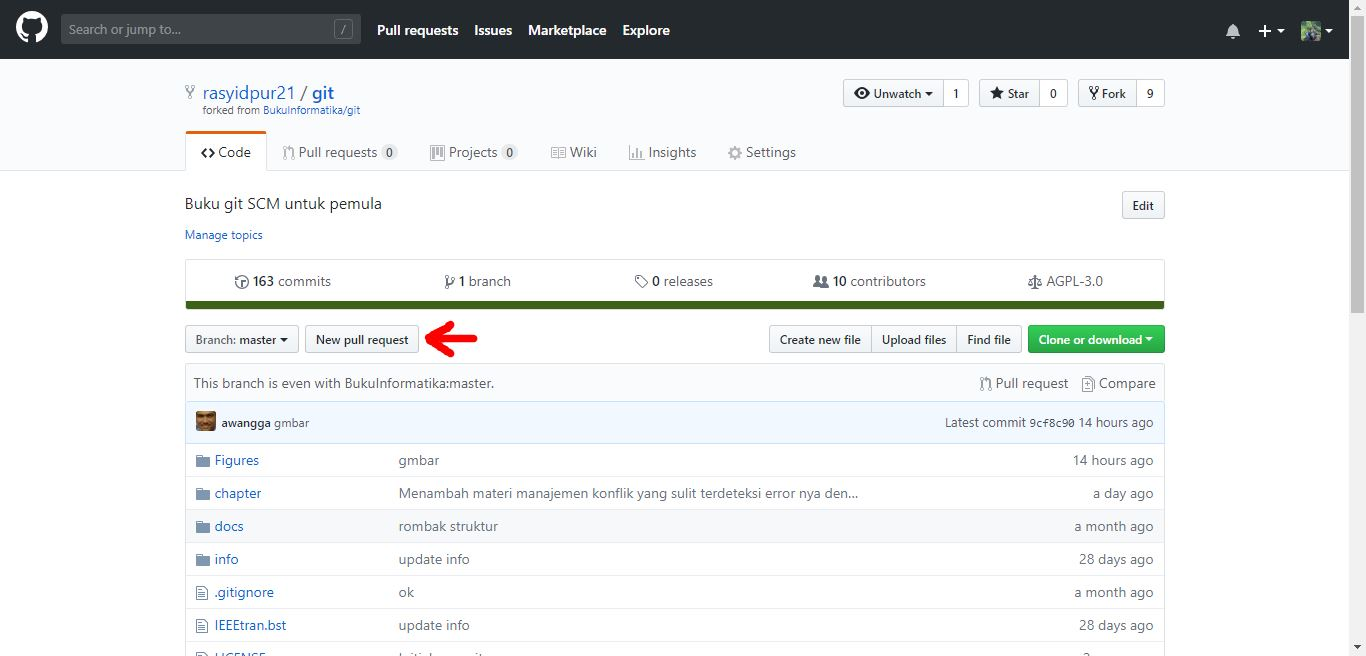
\includegraphics[width=.75\textwidth]{Figures/membacapr/1.JPG}}
\caption{New Pull Request}
\label{fig:newpull}
\end{figure}
\item Setelah itu Github akan melakukan komparasi, apakah kode yang telah dimodifikasi bentrok atau tidak.
\item Jika tidak terjadi bentrok atau konflik biasanya akan muncul notifikasi "\textit{Able to Merge}"
\item Selanjutnya pilih button \textbf{Create Pull Request} seperti pada gambar \ref{fig:create}
\subitem
\begin{figure}[!htbp]
\centerline{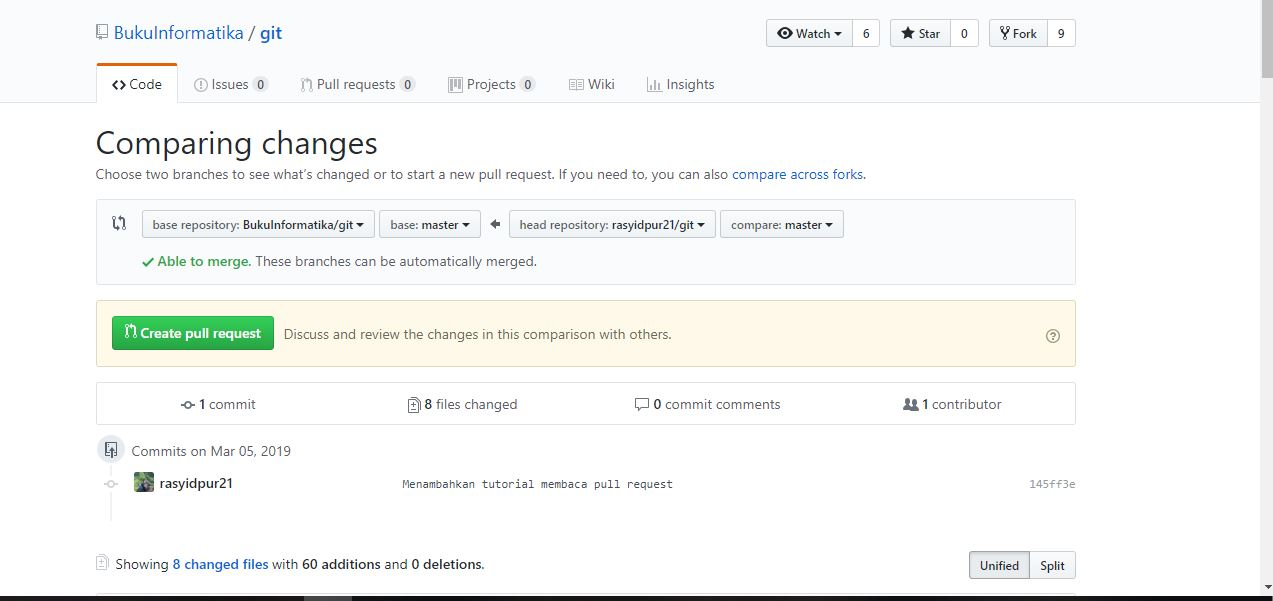
\includegraphics[width=.75\textwidth]{Figures/membacapr/2.JPG}}
\caption{Create Pull Request}
\label{fig:create}
\end{figure}
\item Setelah memilih button \textbf{Create Pull Request} biasanya kita diharuskan mengisi kontribusi apa yang sudah kita lakukan terlebih dahulu, seperti pada gambar \ref{fig:3}
\subitem
\begin{figure}[!htbp]
\centerline{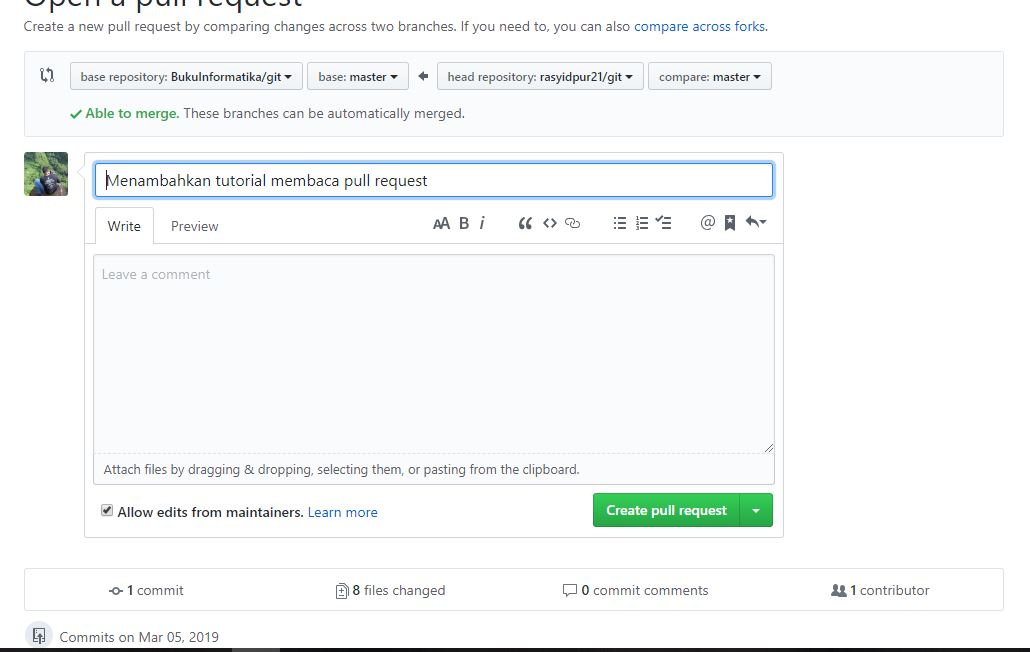
\includegraphics[width=.75\textwidth]{Figures/membacapr/3.JPG}}
\caption{Mengisi Kontribusi}
\label{fig:3}
\end{figure}
\item Selamat!! kita telah berhasil melakukan pull request seperti pada gambar \ref{fig:4}
\subitem
\begin{figure}[!htbp]
\centerline{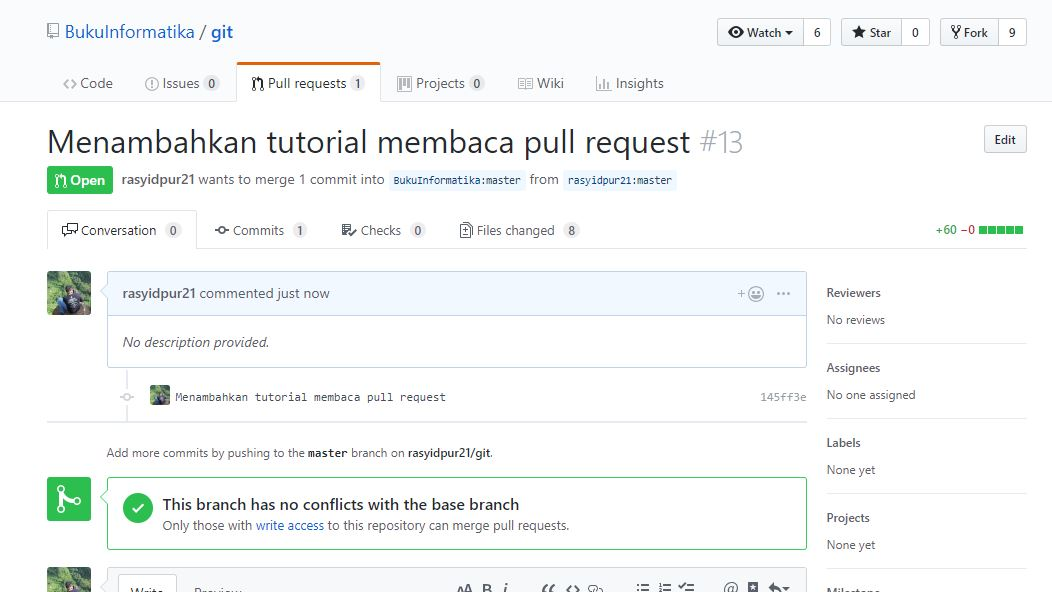
\includegraphics[width=.75\textwidth]{Figures/membacapr/4.JPG}}
\caption{Berhasil Melakukan Pull Request}
\label{fig:4}
\end{figure}
\item Jika telah melakukan pull request admin atau owner akan melakukan review pada kontribusimu apakah akan diterima atau ditolak.
\item Jika kontribusi yang kita lakukan telah diterima, maka akan ada notifikasi yang bertuliskan "\textit{Merged}" yang berwarna ungu seperti pada gambar \ref{fig:merged}
\subitem
\begin{figure}[!htbp]
\centerline{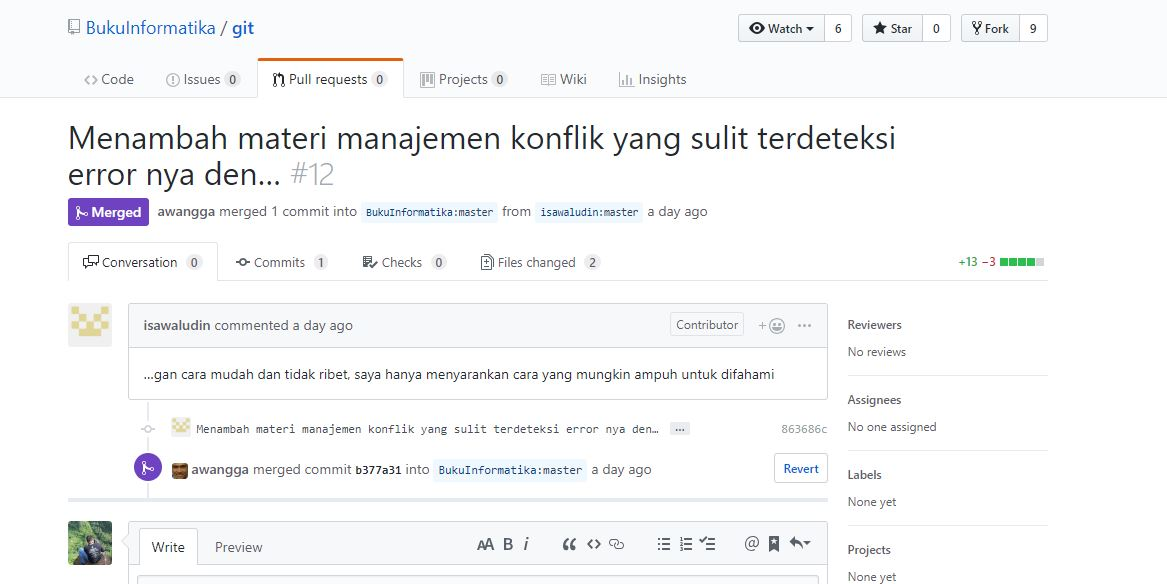
\includegraphics[width=.75\textwidth]{Figures/membacapr/merged.JPG}}
\caption{Kontribusi yang sudah di Merged}
\label{fig:merged}
\end{figure}
\end{enumerate}

Kemudian setelah kita melakukan pull request kita dapat mengetahui kode atau perintah apa saja yang sudah kita perbaharui. Berikut adalah cara membaca pull request yang sudah kita modifikasi :
\begin{enumerate}
\item Buka menu commits pada repository yang kalian kerjakan seperti pada gambar \ref{fig:commits}
\subitem
\begin{figure}[!htbp]
\centerline{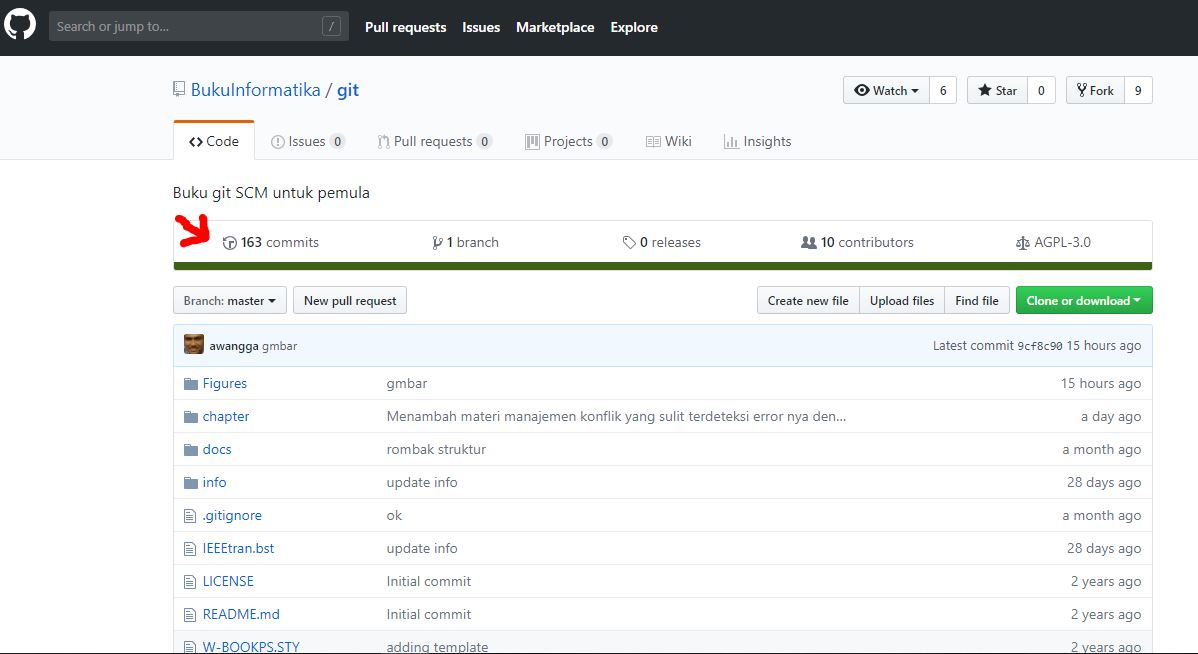
\includegraphics[width=.75\textwidth]{Figures/membacapr/commits.JPG}}
\caption{Menu Commits}
\label{fig:commits}
\end{figure}
\item Kemudian klik kontribusi yang telah kalian lakukan seperti pada gambar \ref{fig:file} 
\subitem
\begin{figure}[!htbp]
\centerline{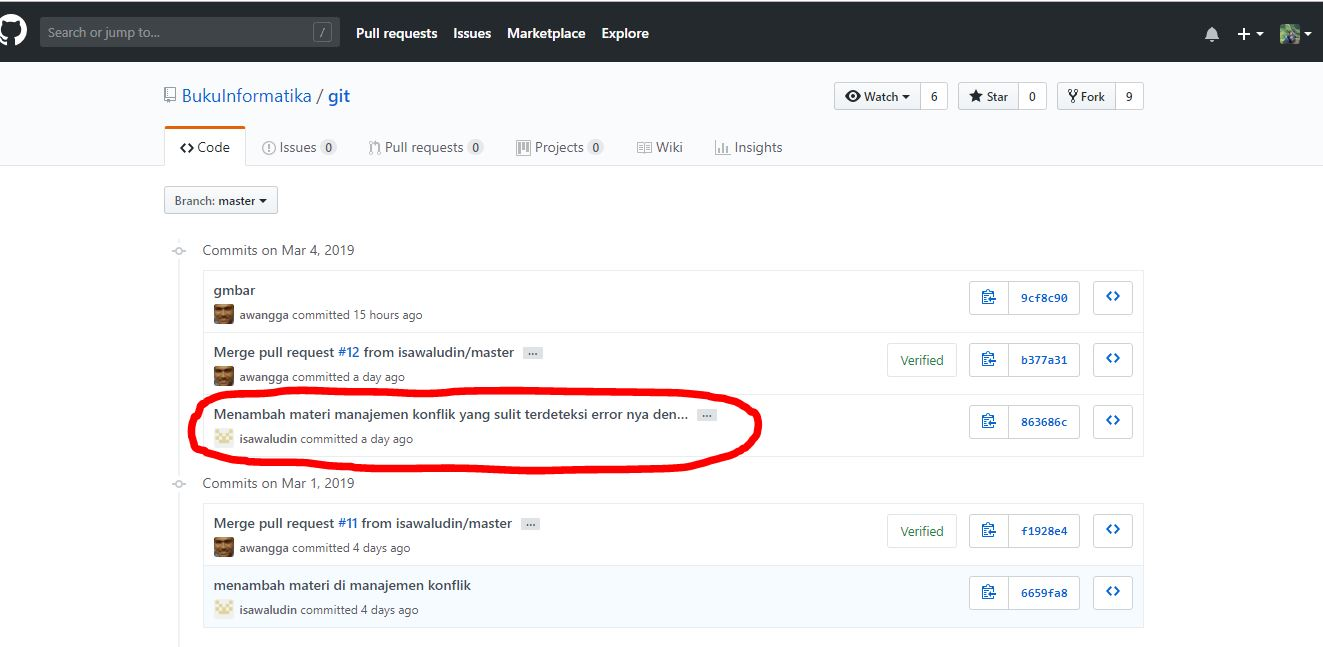
\includegraphics[width=.75\textwidth]{Figures/membacapr/file.JPG}}
\caption{Kontribusi yang telah dilakukan}
\label{fig:file}
\end{figure}
\item Setelah membuka kontribusi yang sudah kita lakukan, kita dapat melihat hal apa saja yang sudah kita perbaharui dalam project yang kita kerjakan. Contohnya seperti pada gambar \ref{fig:line} 
\subitem
\begin{figure}[!htbp]
\centerline{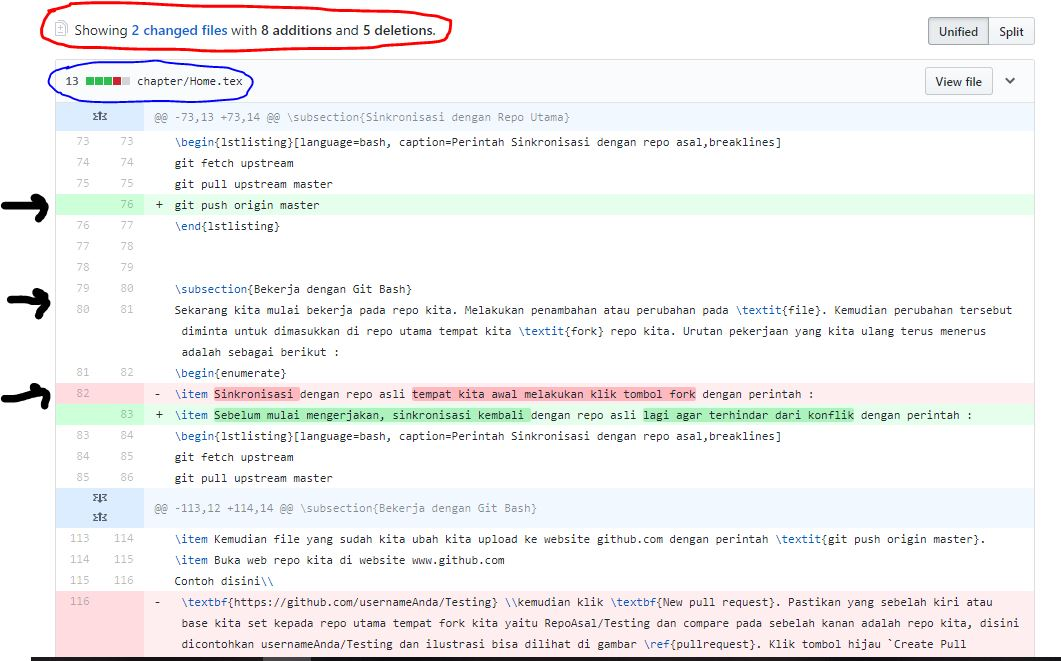
\includegraphics[width=.75\textwidth]{Figures/membacapr/line.JPG}}
\caption{Pull Request yang sudah dilakukan}
\label{fig:line}
\end{figure}
\item Pada gambar \ref{fig:line} di bagian yang di lingkari garis merah terdapat notifikasi "\textit{Showing 2 chages files with 8 additions and 5 deletions}"
\item Arti dari notifikasi tersebut adalah terdapat 2 files yang berubah dengan menambahkan 8 dan menghapus 5 line dalam project yang kita kerjakan
\item Format file yang kita tambahkan, hapus ataupun tetap (tidak berubah) ditandai dengan warna \textbf{hijau}, \textbf{merah} dan \textbf{putih} seperti pada bagian yang dilingkari dengan gari biru pada gambar \ref{fig:line}
\item Line yang berubah dapat kita lihat pada bagian yang ditandai oleh garis hitam
\item Jika line berwarna hijau, artinya ada format yang ditambahkan pada file tersebut
\item Jika line berwarna merah, artinya ada format yang dihapuskan atau dirubah pada file tersebut
\item Jika line berwarna putih, artinya tidak ada format yang berubah pada file tersebut
\end{enumerate}

\section{Standar Untuk Melakukan Approve}
Dalam github orang yang dapat melakukan "\textbf{Approve Merge}" hanyalah  \textbf{Admin} atau \textbf{Owner}. Biasanya admin akan melakukan approve jika kontribusi yang dilakukan oleh seseorang dalam suatu project telah sesuai dengan apa yang dikerjakan dan dengan apa yang dilaporkan.
Pada section ini akan dijelaskan langkah-langkah bagaimana seorang \textbf{Admin} atau \textbf{Owner} menentukan standar untuk melakukan \textbf{Approve} 
\begin{enumerate}
\item Pastikan peserta telah melakukan pull request dalam repository yang telah admin buat
\item Biasanya jika peserta telah melakukan pull request maka admin akan mendapatkan notifikasi di alamat emailnya seperti pada gambar 
\ref{fig:notif}
\subitem
\begin{figure}[!htbp]
\centerline{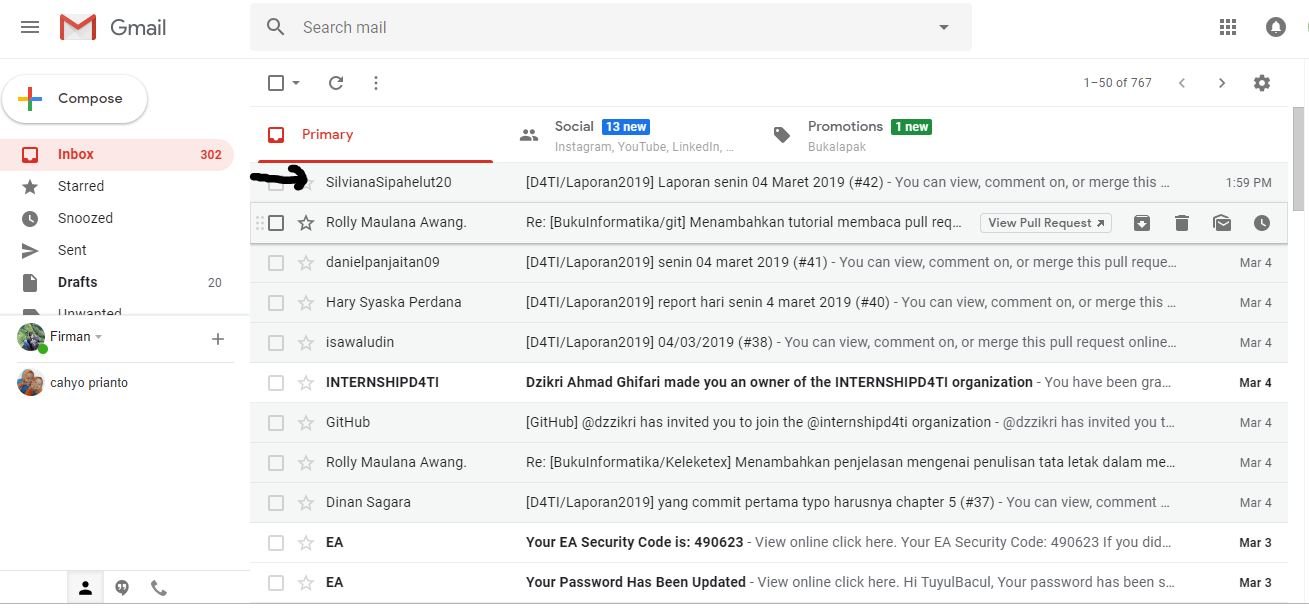
\includegraphics[width=.75\textwidth]{Figures/membacapr/mr1.JPG}}
\caption{Notifikasi Pada Email}
\label{fig:notif}
\end{figure}
\item Kemudian buka notifikasi email tersebut dan klik link untuk melihat pull request yang dilakukan peserta seperti pada gambar \ref{fig:link}
\subitem
\begin{figure}[!htbp]
\centerline{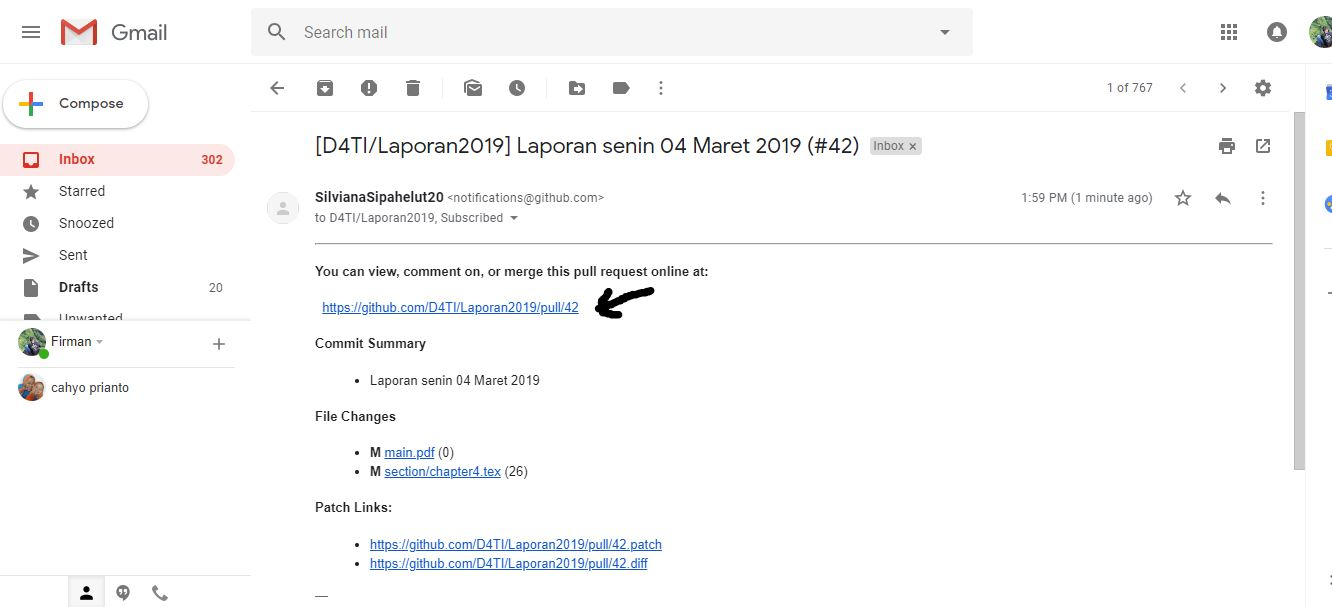
\includegraphics[width=.75\textwidth]{Figures/membacapr/mr2.JPG}}
\caption{View Pull Request Online}
\label{fig:link}
\end{figure}
\item setelah terhubung dengan link github diatas, pilih menu \textbf{File Changed} untuk melihat perubahan apa saja yang telah dilakukan oleh kontributor seperti pada gambar \ref{fig:changed}:
\subitem
\begin{figure}[!htbp]
\centerline{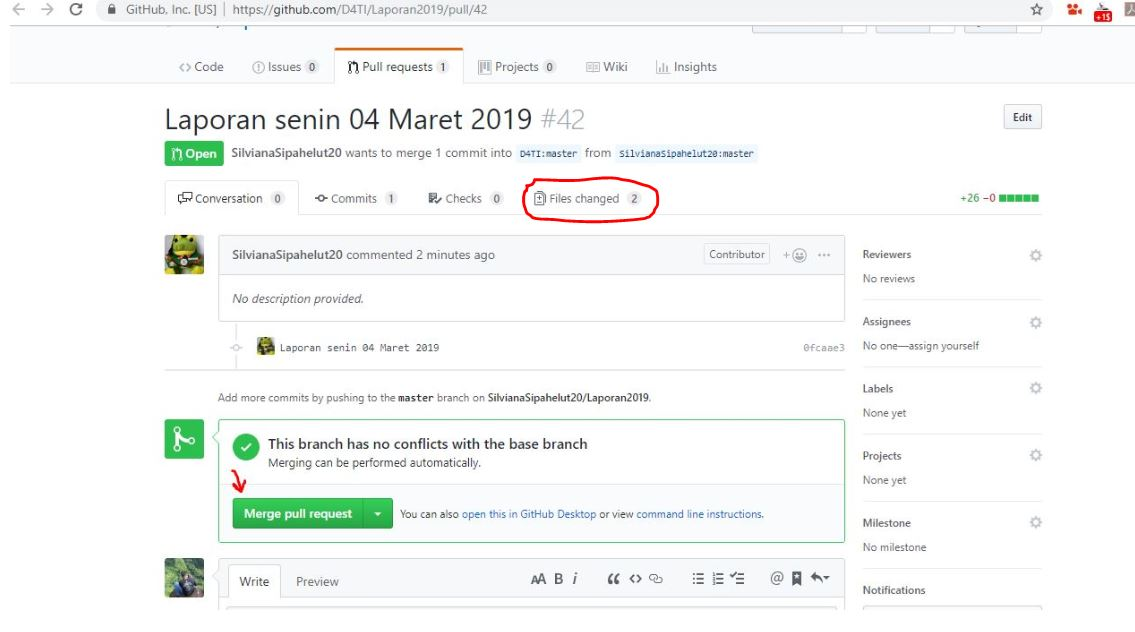
\includegraphics[width=.75\textwidth]{Figures/membacapr/changed.JPG}}
\caption{Melihat Files Changed}
\label{fig:changed}
\end{figure}
\item Setelah itu kita akan melihat apa saja yang telah dimodifikasi oleh kontributor seperti pada gambar \ref{fig:files}:
\subitem
\begin{figure}[!htbp]
\centerline{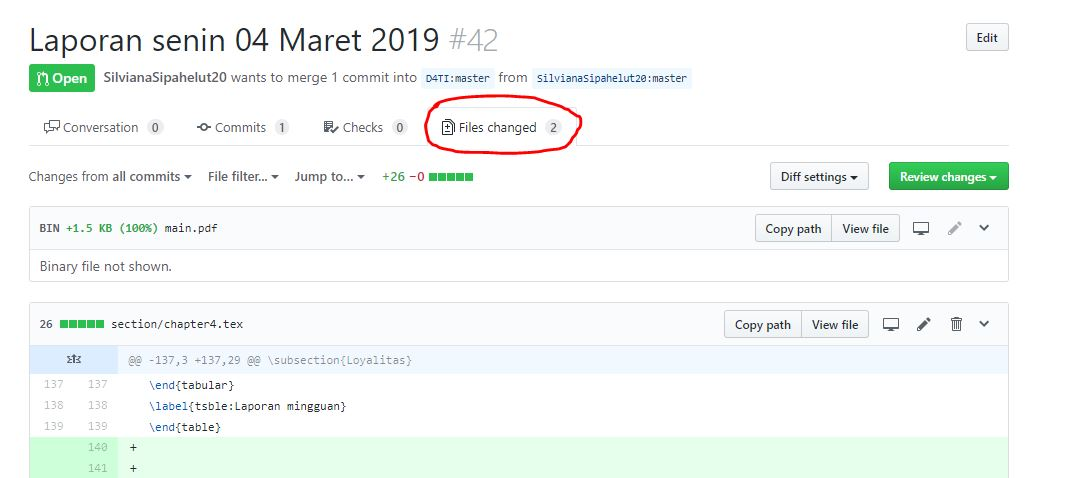
\includegraphics[width=.75\textwidth]{Figures/membacapr/mr7.JPG}}
\caption{File Kontribusi}
\label{fig:files}
\end{figure}
\item Dari perubahan yang telah dilakukan, pastikan bahwa isi dari apa yang dilaporkan kontributor sesuai dengan modifikasi atau perubahan yang telah dia lakukan pada project tersebut
\item Setelah itu admin dapat kembali ke halaman sebelumnya untuk melakukan merging
\item Jika file yang di rubah sesuai maka admin dipersilahkan memilih button \textit{Merge Pull Request} seperti pada gambar \ref{fig:mergepull}
\subitem
\begin{figure}[!htbp]
\centerline{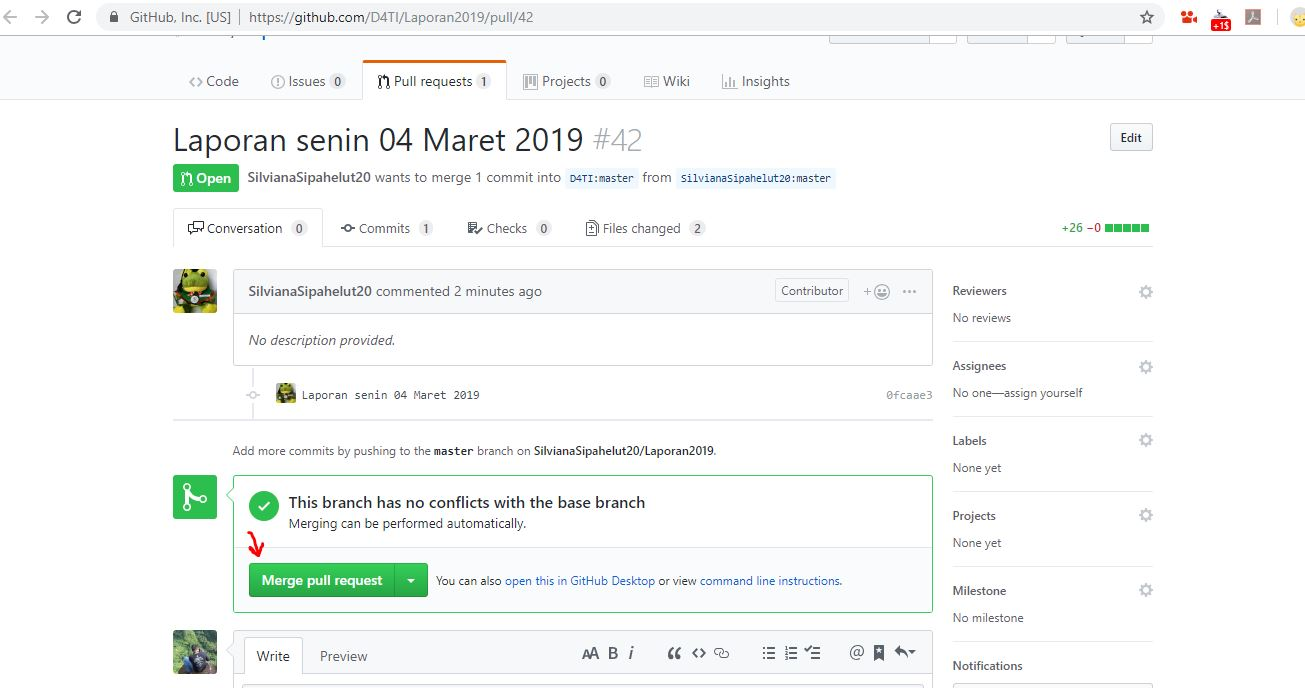
\includegraphics[width=.75\textwidth]{Figures/membacapr/mr3.JPG}}
\caption{Merge Pull Request}
\label{fig:mergepull}
\end{figure}
\item Jika isi kontribusi tidak sesuai admin dapat memilih button \textbf{Close Pull Request} dan memberikan komentar mengenai hal yang harus diperbaiki pada button \textbf{Comment} seperti pada gambar \ref{fig:closed}:
\subitem
\begin{figure}[!htbp]
\centerline{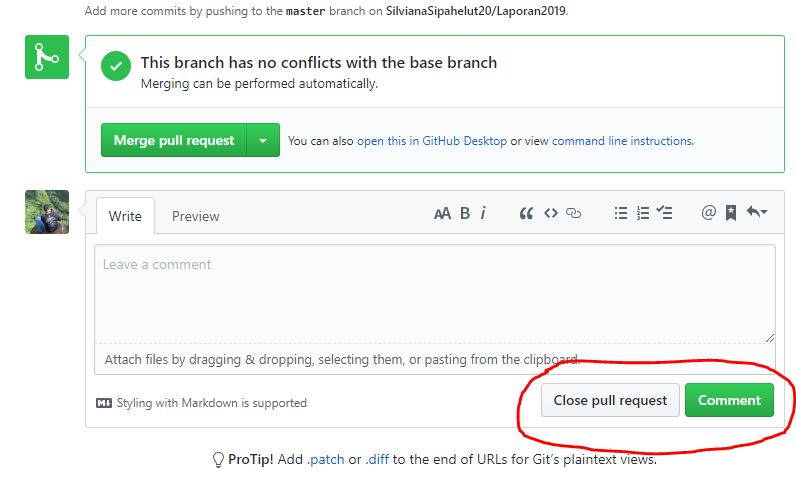
\includegraphics[width=.75\textwidth]{Figures/membacapr/mr4.JPG}}
\caption{Closed and Comment}
\label{fig:Closed}
\end{figure}
\item Setelah itu langkah selanjutnya adalah mengklik button \textbf{Confirm Merge} untuk melakukan konfirmasi seperti pada gambar \ref{fig:confirm}
\subitem
\begin{figure}[!htbp]
\centerline{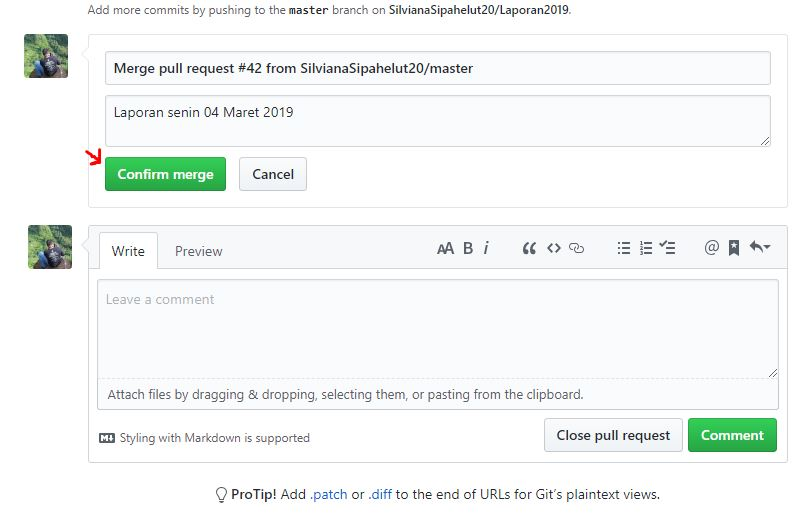
\includegraphics[width=.75\textwidth]{Figures/membacapr/mr5.JPG}}
\caption{Confirm Merge}
\label{fig:confirm}
\end{figure}
\item Setelah melakukan langkah-langkah tersebut, admin telah berhasil melakukan Approve dengan Merge Pull Request seperti pada gambar \ref{fig:approvepull}
\subitem
\begin{figure}[!htbp]
\centerline{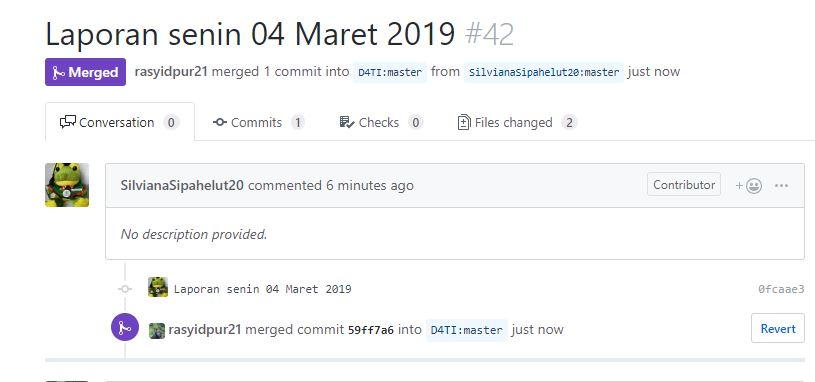
\includegraphics[width=.75\textwidth]{Figures/membacapr/mr6.JPG}}
\caption{Approved Merge Pull Request}
\label{fig:approvepull}
\end{figure}
\end{enumerate}